\chapter{Magnetostatic field calculation 3D}
In general, the magnetostatic field is connected to the magnetization $ [\overrightarrow{M}] $ through the magnetizing tensor [\textbf{TG}].


  The evaluation of the magnetostatic field of a given cell requires the summation on all cells of the mesh due to the the long range of the dipole interaction.
  
  \begin{equation} \label{3d_formula}
  	\overrightarrow{H}(ijk)=-M_{s}\sum\limits_{i'=1}^{N_{x}} \sum\limits_{j'=1}^{N_{y}}\sum\limits_{k'=1}^{N_{z}}\begin{bmatrix}
  	TG_{xx} & TG_{xy} & TG_{xz}\\
  	TG_{yx} & TG_{yy}& TG_{yz}    	\\
  	TG_{zx}&TG_{zy} & TG_{zz}  
  	\end{bmatrix}_{(i-i',j-j',k-k')}\begin{bmatrix}
  	m_{x}\\
  	m_{y}\\
  	m_{z}\end{bmatrix}_{(i',j',k')}
  \end{equation}
  
\begin{figure}[h]
	\centering
	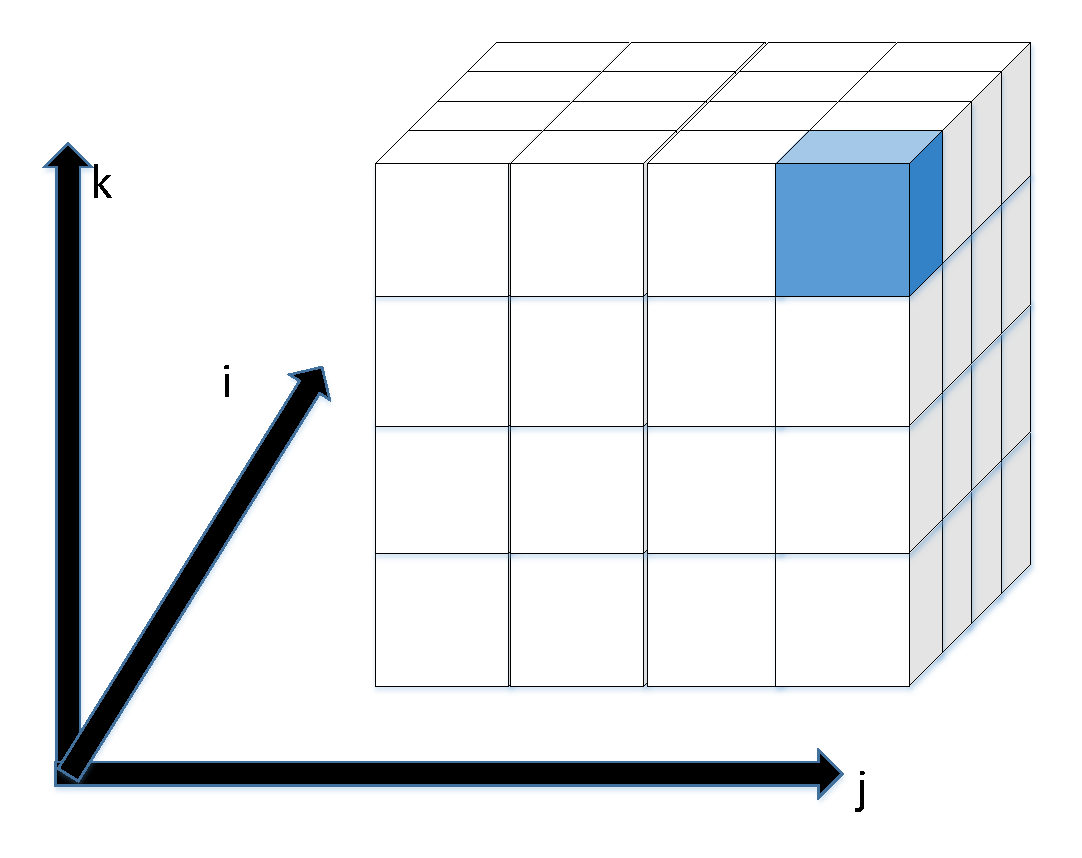
\includegraphics[width=0.7\textwidth]{imm/3d/cube.pdf}  
	\caption{The selected cell is supposed to sum all the magnetostatic field contributions between it and all the other cells}
	\label{fig:cube}
\end{figure}
  
  \clearpage
  \section{Product TG and M}
  Each cell $ (i'j'k') $ has a finite state machine that evaluates the magnetostatic field contribution between the cell \textit{ijk} and the cell \textit{i'j'k'}.
  \begin{center}
  		$ \overrightarrow{h}(i-i',j-j',k-k')= \begin{bmatrix}
  	TG_{xx} & TG_{xy} & TG_{xz}\\
  	TG_{yx} & TG_{yy}& TG_{yz}    	\\
  	TG_{zx}&TG_{zy} & TG_{zz}  
  	\end{bmatrix}_{(i-i',j-j',k-k')}\begin{bmatrix}
  	m_{x}\\
  	m_{y}\\
  	m_{z}\end{bmatrix}_{(i',j',k')}$
  \end{center}.
  
  The matrix \textbf{TG}$ _{(i-i',j-j',k-k')} $ is the magnetizing tensor between the 2 cells, while $ \overrightarrow{M}_{(i',j'k')} $ is the magnetization of the cell $ i',j',k'$.\\\\
  The FSM is composed by the following states:
  \begin{itemize}
  	 \item \textbf{READ\_MX}: save $ m_x $ value
  	 \item \textbf{READ\_MY}: save $ m_y $ value
  	 \item \textbf{READ\_MZ}: save $ m_z $ value
  	 \item \textbf{READ\_TGxx}: read $ TG_{xx} $ value and computing $ op1= TG_{xx}\cdot m_x$
  	 \item \textbf{READ\_TGxy}: read $ TG_{xy} $ value and computing $ op2= TG_{xy}\cdot m_y$
  	 \item \textbf{READ\_TGxz}: read $ TG_{xz} $ value and computing $ h_x= TG_{xz}\cdot m_z +op1+op2$
  	 \item \textbf{READ\_TGyx}:read $ TG_{yx} $ value and computing $ op1= TG_{yx}\cdot m_x$
  	 \item \textbf{READ\_TGyy}:read $ TG_{yy} $ value and computing $ op2= TG_{yy}\cdot m_y$
  	 \item \textbf{READ\_TGyz}: read $ TG_{yz} $ value and computing $ h_y= TG_{yz}\cdot m_z +op1+op2$
  	 \item \textbf{READ\_TGzx}:read $ TG_{zx} $ value and computing $ op1= TG_{zx}\cdot m_x$
  	 \item \textbf{READ\_TGzy}:read $ TG_{zy} $ value and computing $ op2= TG_{zy}\cdot m_y$
  	 \item \textbf{READ\_TGzz}: read $ TG_{zz} $ value and computing $ h_z= TG_{zz}\cdot m_z +op1+op2$
  \end{itemize}
   
     \section{Logic Plane}
     This component group all the cells in a given plane, and enable the computation of the magnetostatic field contributions between the cell \textit{ijk} and the all the cells in a given plane (i.e. k is fixed).
     \begin{center}
     	$ \overrightarrow{h}(i-i',j-j',k-k^*)$\quad \quad $ \forall i'<N_x,$ $ j'<N_y,$ $ k=k^* $
     \end{center}
          All this computation can be done in parallel.
    \section{Sum all}
    The \textit{sum\_all} is a component that given a fixed $ k^* $ (i.e. a given plane) evaluates the magnetostatic field of all cells in a fixed plane.
    The input is given by the \textit{logic plane}
    \begin{center}
    	$ \sum\limits_{i'=1}^{N_{x}} \sum\limits_{j'=1}^{N_{y}}\begin{bmatrix}
    	TG_{xx} & TG_{xy} & TG_{xz}\\
    	TG_{yx} & TG_{yy}& TG_{yz}    	\\
    	TG_{zx}&TG_{zy} & TG_{zz}  
    	\end{bmatrix}_{(i-i',j-j',k-k^*)}\begin{bmatrix}
    	m_{x}\\
    	m_{y}\\
    	m_{z}\end{bmatrix}_{(i',j',k^*)} $
    \end{center}
    By looking to the formula \ref{3d_formula}, we have to evaluate the sum for each plane, so we store this sum and wait for the next plane to be computed and added to the previous sum.\\
    Of course when we reach the $ k^{th} $ plane, we stop the sum and we set a signal to tell that the calculation is finished.
  